\documentclass[10pt]{article}
\usepackage[utf8]{inputenc}
\usepackage[T1]{fontenc}
\usepackage[margin=0.9in]{geometry}
\usepackage{amsmath,amssymb,amsthm}
\usepackage{booktabs}
\usepackage{array}
\usepackage{url}
\usepackage{microtype}
\usepackage{graphicx}
\usepackage{caption}
\usepackage{xcolor}
\usepackage{listings}
\usepackage{enumitem}
\usepackage{seqsplit}
\usepackage[hidelinks]{hyperref}
\makeatletter\g@addto@macro{\UrlBreaks}{\do\_\do\.\do\/}\makeatother
\emergencystretch=3em
\tolerance=2000
\setlist{itemsep=1pt,topsep=2pt,parsep=0pt}
% generated by gen_inputs.py; do not edit
\newcommand{\SSAShaMain}{35add509990d50ebbdbbb70476fc652867d236a62534eda3d1021a414c21ae4d}
\newcommand{\SSAShaCtl}{aa94aca898a83529624931dd73dc7f0a3ab0ab31e78c9393de8c597661613895}
\newcommand{\SSAShaRegion}{38974cc16e90e77ac1553bedf6907ff2eb53f7689df00a9a82668d11574f0421}
\newcommand{\SSAShaMatch}{match}
\newcommand{\SSACompileMain}{rc 0 in 7.8~s (stage S3: rc 0 in 8.4~s)}
\newcommand{\SSACompileCtl}{rc 0 in 4.6~s (stage S3: rc 0 in 4.9~s)}
\newcommand{\SSAAxiomsSame}{identical}
\newcommand{\SSACtlSame}{identical}
\newcommand{\SSALockCheck}{match: true}
\newcommand{\SSANDefsLines}{112}
\newcommand{\SSAPairsEqual}{22}
\newcommand{\SSAPairsTotal}{22}
\newcommand{\SSARecordSha}{90e4f4055ce7f589303ad246dac23845db75f397aecbad71533230e34a86ee01}
\newcommand{\SSAPosElapsed}{490.35}
\newcommand{\SSAPosChild}{478.001}
\newcommand{\SSATInitCore}{220.1}
\newcommand{\SSATCalcLam}{2.8}
\newcommand{\SSATCalcK}{0.3}
\newcommand{\SSATBdsup}{23.6}
\newcommand{\SSATGlobalGrid}{125.4}
\newcommand{\SSATInsideHess}{105.7}
\newcommand{\SSAPosExe}{ca7b5cae54a79c684f08c696a8a182fd9e4d9567701f6975596a26ac2dcddf1f}
\newcommand{\SSAPosLog}{cf6cc0c6fdf8175af35933f9000dfe8cca7edc5714e4922c152b011acb5208f8}
\newcommand{\SSAPosStart}{2026-10-25 20:23:19 UTC}
\newcommand{\SSAPosEnd}{2026-10-25 20:31:30 UTC}
\newcommand{\SSAPosStages}{passed}
\newcommand{\SSAPosUnchanged}{true}
\newcommand{\SSACompiler}{g++ (Ubuntu 11.4.0-1ubuntu1~22.04.3) 11.4.0}
\newcommand{\SSAPython}{3.10.12}
\newcommand{\SSAShaCert}{53d46bba38d671690b07b9893ea08feb5bdcea8039280c609be783f9e66a3bb2}
\newcommand{\SSAShaCore}{c7f76596cde648ae35707a242406a6b02d6b41bad6b19123aeca3aaec47dced3}
\newcommand{\SSAShaGrids}{4640e0a32eb20071800d408fc2b7b47269cdfcecfa99c862940c7afbbdaaa50b}
\newcommand{\SSAShaRun}{cbef4f4c082102a826e4b92c298c94fdfe3b5ff6622702b6226478142e1c7075}
\newcommand{\SSAElneg}{683}
\newcommand{\SSARcneg}{-6}
\newcommand{\SSATokneg}{false}
\newcommand{\SSAStgneg}{failed}
\newcommand{\SSAElA}{1009}
\newcommand{\SSARcA}{0}
\newcommand{\SSATokA}{true}
\newcommand{\SSAStgA}{passed}
\newcommand{\SSAElB}{874}
\newcommand{\SSARcB}{-6}
\newcommand{\SSATokB}{false}
\newcommand{\SSAStgB}{failed}
\newcommand{\SSAErMid}{5.52}
\newcommand{\SSAErInt}{9.48}
\newcommand{\SSAMstar}{22.6}
\newcommand{\SSAFactorAPred}{20.5}
\newcommand{\SSAFactorAObs}{20}
\newcommand{\SSAMdrop}{1.86}
\newcommand{\SSABPred}{758}
\newcommand{\SSABObs}{758}
\newcommand{\SSASlack}{4585}
\newcommand{\SSAAllow}{5343}
\newcommand{\SSACalLo}{-4.15042142}
\newcommand{\SSACalHi}{-4.15040429}
\newcommand{\SSAWtri}{-4.1504128076789633794}
\newcommand{\SSACalWidth}{1.71265e-5}
\newcommand{\SSACalOffLo}{-8.61e-06}
\newcommand{\SSACalOffHi}{8.52e-06}
\newcommand{\SSANegSquare}{-4.11716061233}
\newcommand{\SSANegNoTwoPi}{-0.201089447612}
\newcommand{\SSANegShift}{-1.26348226266}
\newcommand{\SSAEwaldDiff}{2.1382e-50}
\newcommand{\SSASSTri}{-0.20108945}
\newcommand{\SSASSSq}{-0.1957972}
\newcommand{\SSACdiff}{4.0091e-51}
\newcommand{\SSAReLam}{-6.73002928856}
\newcommand{\SSAReMu}{0.413883384579}
\newcommand{\SSAReK}{-0.00348158666}
\newcommand{\SSAReG}{1.008\times10^{-53}}
\newcommand{\SSAReId}{-1.034\times10^{-25}}
\newcommand{\SSAReNoAngLam}{-6.752949}
\newcommand{\SSAReNoAngK}{-0.0039749}
\newcommand{\SSAReDropLam}{-6.765096}
\newcommand{\SSAReDropK}{0.0005261}
\newcommand{\SSABl}{1.04646435626}
\newcommand{\SSAClOne}{0.634692}
\newcommand{\SSABlNegA}{1.0827}
\newcommand{\SSABlNegB}{1.0278}
\newcommand{\SSALFPosAcc}{13}
\newcommand{\SSALFPosN}{13}
\newcommand{\SSALFNegAcc}{7}
\newcommand{\SSALFNegN}{10}
\newcommand{\SSALFFailedList}{\texttt{gmin - factor > 0 (m\_* - E\_0 - E\_I > 0)}; \texttt{m\_* - E\_0 - E\_I >= 1.20e-5}; \texttt{gmin.lo - factor.hi > 0 on printed pairs}}
\newcommand{\SSALFNFailed}{3}
\newcommand{\SSALFCommit}{84e0c2899830fba671022eefcd408af9ecd565c8}
\newcommand{\SSALFLean}{Lean 4.34.1}
\newcommand{\SSALFBranch}{feat/lean-data-certificates-2026-10-25}
\newcommand{\SSALFPassed}{88}
\newcommand{\SSALFPytestTime}{21.72}
\newcommand{\SSALFPinnedLog}{4 passed, 84 deselected}
\newcommand{\SSALFNotPinned}{84}
\newcommand{\SSALFNNew}{6}
\newcommand{\SSALFOldCommit}{542cea97aa78e30d8935ec81278aeb697a9f5dc7}
\newcommand{\SSALFFixCommit}{2c168be2de8104dddc48daecee1423c8d8f076b7}
\newcommand{\SSAShaMainOld}{d899416e3ed4189b10342e346a50454c629d4fffea057fe8a48ea19bf17476ff}
\newcommand{\SSAnR}{10}
\newcommand{\SSAnG}{7}
\newcommand{\SSAnK}{8}
\newcommand{\SSAnT}{6}
\newcommand{\SSAnSteps}{31}
\newcommand{\SSALedgerN}{25}
\newcommand{\SSALedgerA}{7}
\newcommand{\SSALedgerL}{5}
\newcommand{\SSALedgerC}{5}
\newcommand{\SSALedgerX}{8}
\newcommand{\SSAGateExit}{1}
\newcommand{\SSAGateFlag}{7}
\newcommand{\SSAGateBlock}{0}
\newcommand{\SSAGateOther}{0}

\lstset{basicstyle=\ttfamily\scriptsize,columns=fullflexible,keepspaces=true,breaklines=true,
  frame=single,framesep=2pt,xleftmargin=3pt,xrightmargin=3pt,upquote=true,
  keywordstyle=\bfseries,morekeywords={theorem,lemma,def,noncomputable,abbrev,where,fun,Prop,axiom,namespace,open,scoped},
  escapeinside={(*@}{@*)}}
\newcommand{\R}{\mathbb{R}}
\newcommand{\tier}[1]{\textsf{[#1]}}
\newcommand{\lean}[1]{\texttt{#1}}
\newcommand{\hash}[1]{\texttt{\expandafter\seqsplit\expandafter{#1}}}
\newcommand{\leanl}[1]{\par\smallskip\noindent\fbox{\parbox{\dimexpr\linewidth-2\fboxsep-2\fboxrule\relax}{\footnotesize\textsf{Lean counterpart.} #1}}\par\smallskip}
\newcommand{\curl}{\operatorname{curl}}
\renewcommand{\div}{\operatorname{div}}
\makeatletter\newcommand{\tabinput}[1]{\@@input #1 }\makeatother

\title{The Sandier--Serfaty triangular-lattice conjecture:\\
an independent reproduction of a claimed finite certificate,\\
an adversarial audit of the claimed reduction, and a Lean statement\\[2pt]
{\large (no proof of the conjecture is claimed)}}
\author{Xavier Callens (SocrateAI Lab)}
\date{Preprint v1, 2026-10-25 \quad (not peer reviewed)}
\hypersetup{pdftitle={Sandier-Serfaty conjecture: reproduction of a finite certificate, audit of the reduction, Lean statement},
  pdfauthor={Xavier Callens}}

\begin{document}
\maketitle

\noindent\textbf{AI-assistance disclosure.} This preprint, its Lean code, its Python and C++ harness code, the LeanFlow
generator and the claim ledger were produced by AI agents (Claude, Anthropic) under the author's direction. The author is
responsible for the content. No human has audited the Lean statements for adequacy, no human referee has checked the
hand arguments, and every ``independent'' check below is made by an agent of the same AI pipeline as the producer, never by
a person. The mathematics under study was itself produced by an AI system (the openai/math release) and is not peer
reviewed. \emph{Revision note.} This version incorporates the corrections required by an independent audit by a second agent
instance of the same pipeline (misreported number in Section~\ref{sec:num}(b), fail-open LeanFlow checker for foreign sources
in Section~\ref{sec:lf}, conditional wording of Step~10, and non-blocking items); \texttt{AUDIT.md} and \texttt{REVISION.md}
are in the paper directory.

\begin{abstract}
The Sandier--Serfaty conjecture asks whether the triangular lattice minimizes the renormalized Coulomb energy $W$ of a
point set in the plane against a uniform neutralizing background~\cite{ss}. A preprint in the openai/math release
\cite{oai} (AI-generated, not peer reviewed) claims a proof, by a reduction to square tori plus a finite certificate in
exact interval arithmetic. We do \emph{not} prove or verify that claim. We report three things.
\textbf{(1) Independent reproduction of the finite certificate} \tier{X}: the unchanged C++ certificate was re-executed
on a different toolchain and host (\texttt{\SSACompiler}, Python~\SSAPython); the wrapper exited~0, the terminal line was
\texttt{OK}, source hashes were unchanged, and all \SSAPairsEqual{} of \SSAPairsTotal{} printed integer pairs equal the saved
record. Three one-line loosenings of the certificate were run as negative controls: two are rejected by the program's own
assertion and one passes (the outcomes of the last two were predicted in writing before they finished). The reproduction rests on the manuscript's analytic bounds and
tests none of them.
\textbf{(2) Adversarial audit of the reduction} \tier{C}: by an AI agent, Sections 2--5 were checked step by step
(\SSAnSteps{} numbered steps, 14 certificate-stage rows); no step was classified as a gap, with stated limits (the
spline pieces outside $[p,R_0]$, the grid-stage values, and runtime trust are not independently checked). This is not a proof and not peer review.
\textbf{(3) A Lean statement} \tier{A for non-degeneracy lemmas only, C for fidelity}: the conjecture is stated as Lean
\lean{Prop}s (manuscript and Sandier--Serfaty normalizations, plus the explicit value); ten non-degeneracy lemmas are
kernel-checked within the axioms $\{\lean{propext},\lean{Classical.choice},\lean{Quot.sound}\}$, planted
\lean{sorry} and planted-axiom controls are caught; the statements themselves are \emph{not proved}.
We also add a Lean data-certificate generator to the LeanFlow project (\SSALFPassed{} tests pass), fail-closed for the sources it renders itself, which accepts
the arithmetic of the positive run's printed pairs and rejects that of the loosened run. An independent audit found that the exported checker
for \emph{arbitrary} Lean sources was fail-open (a source using \lean{\#exit} and a forged axiom report was accepted); this is fixed in the
checker (Section~\ref{sec:lf}). Nothing here shows that the conjecture holds.
\end{abstract}

\paragraph{Tiers.} \tier{A}: kernel-checked Lean, axioms within the allowlist, planted controls caught; a Tier~A tag attaches to the
Lean statement, never to its gloss. \tier{L}: a cited source whose statement we read on the cited page (proofs not re-checked).
\tier{C}: a human-style argument not machine-checked (here: by an agent). \tier{X}: computation, including exact-integer and
exact-rational computation whose toolchain is trusted; it never supports a mathematical claim by itself. Identifiers
\texttt{SSA-A-0001} etc.\ refer to \texttt{ledger/ledger.json} (Section~\ref{sec:ledger}). Everything resting on the openai/math
manuscript is conditional on it.

\section{Setting, and what is and is not claimed}\label{sec:setting}
For $R>1$ let $K_R=[-R,R]^2$ and fix cutoffs $\chi_R\in C_c^\infty(\R^2)$ with $0\le\chi_R\le1$, $\operatorname{supp}\chi_R\subset K_R$,
$\chi_R=1$ on $K_{R-1}$ and $\sup_R\|\nabla\chi_R\|_\infty<\infty$. For a locally finite point set $\Lambda$ with
$\nu_\Lambda=\sum_{p\in\Lambda}\delta_p$ and bounded density $\sup_R\nu_\Lambda(B_R)/|B_R|<\infty$, the admissible class
$\mathcal A_1$ consists of locally integrable fields $E$ with
\begin{equation}\label{eq:adm}\div E=2\pi(\nu_\Lambda-1),\qquad \curl E=0\quad\text{in distributions.}\end{equation}
The renormalized energy is
\begin{equation}\label{eq:W}
W(E,\chi_R)=\lim_{\eta\downarrow0}\Bigl[\tfrac12\!\int_{\R^2\setminus\bigcup_pB(p,\eta)}\!\chi_R|E|^2+\pi\log\eta\sum_{p\in\Lambda}\chi_R(p)\Bigr],\qquad
W(E)=\limsup_{R\to\infty}\frac{W(E,\chi_R)}{4R^2},
\end{equation}
and $\Lambda_\triangle=\sqrt{2/\sqrt3}\,(\mathbb Z(1,0)+\mathbb Z(\tfrac12,\tfrac{\sqrt3}2))$ has covolume one, with $E_\triangle=-\nabla h_\triangle$
the field of the mean-zero periodic solution of $-\Delta h_\triangle=2\pi(\delta_0-1)$ on $\R^2/\Lambda_\triangle$. These are the
definitions of the manuscript~\cite{oai} (its eqs.\ for cutoffs, admissibility, local and whole energy), which follow
Sandier--Serfaty~\cite{ss} \tier{L, SSA-L-0003}. The \textbf{conjecture} (SS2012 Conjecture~1, p.~5) is $W(E)\ge W(E_\triangle)$ for every $E\in\mathcal A_1$;
SS2012 prove it among lattices (Theorem~2) and state that ``its minimization in general remains open'' \tier{L, SSA-L-0001}.
Betermin--Sandier~\cite{bs} show that it is equivalent to the Brauchart--Hardin--Saff value of the next-order term of the optimal
logarithmic energy of $N$ points on $S^2$~\cite{bhs} \tier{L, SSA-L-0004, SSA-L-0005}. The manuscript~\cite{oai} claims
$W(E)\ge W(E_\triangle)$ and hence that sphere value.

\paragraph{What this paper does.} It (i) re-executes the manuscript's finite certificate and attacks it with negative controls
(Section~\ref{sec:num}); (ii) audits the reduction that feeds the certificate (Section~\ref{sec:human}, summarized in
Section~\ref{sec:audit}); (iii) states the conjecture in Lean (Section~\ref{sec:lean}); (iv) improves LeanFlow, our Lean tooling,
with a generator that turns printed interval data into Lean-checked arithmetic and fails closed on the sources it renders itself (Section~\ref{sec:lf}; the audit-found hole in the checker for foreign sources and its fix are reported there). The
rusty-SUNDIALS numerical library is not needed for this lane (the certificate is exact integer arithmetic, not an ODE problem).
\paragraph{What it does not do.} It does not prove, verify or refute the conjecture, it is not peer review, and it did not search
the literature for resolutions after the cited papers (the status ``open'' is that of the cited sources). A reproduction of an
exact-integer computation shows that the program, as written, behaves as recorded on a second toolchain; whether it certifies
the analytic inequalities it is meant to certify is an audit question (Section~\ref{sec:audit}), not a computing one.

\section{Step-by-step human demonstration of the claimed argument}\label{sec:human}
This section is for a reader who knows the notation of Section~\ref{sec:setting}. It restates, step by step, the argument of
the manuscript \emph{as re-derived by the audit agent}; it is not our proof, and each step carries (a) the audit's tier, (b) the
audit rows (R/G/K/T) and ledger id, and (c) the matching Lean statement, which for most steps is ``none''. The only parts
with Lean content are the definitions (Step~0), the value (Step~7) and the target statement (Step~10), plus the data certificates (Step~9).
The logical shape is: Steps 1--4 reduce $W(E)$ on the plane to a lower bound $\mathcal W_n(h)\ge nC$ on square tori $T_n=\R^2/(\sqrt n\,\mathbb Z^2)$; Steps 5--9 are the manuscript's argument for that torus bound with
$C=W(E_\triangle)$; Step~10 concludes.

\paragraph{Step 0: the objects \tier{L, SSA-L-0003}.} $\mathcal A_1$, $W(E,\chi)$, $W(E)$ and $\Lambda_\triangle$ as in~(\ref{eq:adm})--(\ref{eq:W}).
\leanl{\lean{Admissible}, \lean{AdmissibleBg}, \lean{WeakDivE}, \lean{WeakCurlFree}, \lean{HasLocalEnergy}, \lean{IsSquareCutoffFamily},
\lean{WSq}, \lean{triLattice} (Listing~\ref{lst:defs}). Equations hold weakly against $C_c^\infty$ test functions; the puncture limit is a relation (integrable on the punctured
domain plus \lean{Tendsto}), never \lean{limUnder}. Non-degeneracy, \tier{A, SSA-A-0001..0005}: the class $\mathcal A_1$ is non-empty ($E=-\pi x$, no charges), the background constant is load-bearing
(controls $b=0$, $b=-2\pi$ fail), both cutoff classes are non-empty, and the bases have covolume $1$ and $2\pi/m$.}

\paragraph{Step 1: local structure; the puncture limit exists \tier{C, audit R1}.} Near a charge $p$, $E_p^0=\nabla\log|x-p|-\pi(x-p)$ has $\div E_p^0=2\pi\delta_p-2\pi$ and
$\curl E_p^0=0$; the difference $E-E_p^0$ has vanishing divergence and curl in the sense of distributions, so by Weyl's lemma it is smooth. Hence $E=(x-p)/|x-p|^2+$smooth near $p$,
$E\in L^q_{\rm loc}$ for $q<2$, and $\tfrac12|E|^2-\tfrac1{2|x-p|^2}$ is integrable, which is exactly what makes the limit~(\ref{eq:W}) exist and be finite.
\leanl{Assumed, not proved: \lean{HasLocalEnergy} states the limit as a hypothesis on the competitor. If the limit failed to exist for some admissible $E$, that $E$ would drop out of the competitor class, so the Lean statement would be \emph{weaker} (Section~\ref{sec:lean}). Needs Weyl's lemma, absent from Mathlib at the pinned revision.}

\paragraph{Step 2: normalization bridge \tier{C+L, audit R2, R3; SSA-L-0003, SSA-L-0004}.} Put $j=(-E_2,E_1)$. Then $\div j=-\curl E=0$ and $\curl j=\div E=2\pi(\nu-1)$, so $j$ is an
SS2012 current with background $m=2\pi$. The scaling~(1.9) $j'=m^{-1/2}j(\cdot/\sqrt m)\in\mathcal A_1^{SS}$, $W(j)=m(W(j')-\tfrac14\log m)$ \tier{L, SS2012 p.~3}
has the change of variables $y=\sqrt m\,x$ behind it: the puncture radius becomes $\eta'=\sqrt m\,\eta$, which produces $+\pi\log\sqrt m$ per charge,
so $W(E,\chi_R)=W(j',\xi_t)-\tfrac\pi2\log m\sum_p\xi_t(p)$ with no area factor.
\leanl{\lean{SandierSerfatyStatement} (field $E$, square cutoffs, covolume one) and \lean{SandierSerfatyOriginalStatement} (current $j$, ball cutoffs, $\Lambda_m$ of covolume $2\pi/m$, every $m>0$) are two separate \lean{Prop}s. Their equivalence is \tier{L/C} and is not formalized.}

\paragraph{Step 3: $W(E)>-\infty$ on the plane \tier{C+L, audit R4--R7; SSA-L-0001, SSA-L-0002}.} For $E\in\mathcal A_1$ with $W(E)<\infty$ the local energies and charge counts are $O(t^2)$ on $Q_t$. SS2012 Lemma~4.7 (a Struwe-type dyadic $L^r$ bound,
$1<r<2$) then gives $\int_{Q_{t+A}}|j'|^r\le Ct^2(\log t)^{r/2}$, and Hölder with the coarea formula bounds the number of charges in a strip of width $L$ around $\partial Q_t$ by
$C(t+t^{1+1/r}(\log t)^{1/2})=o(t^2/\log t)$. SS2012 Proposition~4.9 (one measure $g\ge-C$ serving two cutoffs) turns the cutoff change $\xi_t\to\zeta_{Q_{t-L}}$ into an error
$Cn(\log(2+n)+1)=o(t^2)$ with $n$ the strip count. With SS Theorem~1(3) ($\min_{\mathcal A_1}W_U=:M$ finite) this gives $W(E)\ge2\pi(M-\tfrac14\log2\pi)>-\infty$.
\leanl{None. No Lean statement of Lemma~4.7 or Proposition~4.9 exists; both are cited \tier{L} and their proofs are not re-checked.}

\paragraph{Step 4: reduction to square tori \tier{C+L, audit R8--R10; SSA-L-0001}.} For a periodic field the energy per area equals the torus energy over the area (R8). On $T_n$, $E_{T_n}(E)=\mathcal W_n(h)+\tfrac n2|c|^2$ where $E=-\nabla h+c$
(R9): the harmonic part is constant and $\int\nabla h=0$. SS2012 Theorem~1(4) supplies a minimizing sequence $j_k$ for $M$, periodic with respect to axis-aligned squares of side $\sqrt{2\pi N_k}$; rescaling to
$E_k(x)=\sqrt m(j_2,-j_1)(\sqrt m\,x)$ with $m=2\pi$ gives fields on $T_{N_k}$ with $E_T(E_k)/N_k=m(W_{\rm ball}(j_k)-\tfrac14\log m)\to m(M-\tfrac14\log m)$. Hence if $\mathcal W_n(h)\ge nC$ for every $n\ge2$ and every configuration, then $W(E)\ge C$ for all $E\in\mathcal A_1$, and $\inf_{\mathcal A_1}W=W(E_\triangle)$ when $C=W(E_\triangle)$.
\leanl{None (the torus theorem and this reduction are not stated in Lean).}

\paragraph{Step 5: a torus minimizer, separation, Voronoi sectors \tier{C, audit G1--G3}.} (G1) $\mathcal W_n=\pi nR_n+\pi\sum_{i\ne j}G_n(v_i-v_j)$ (Green's identity; each site contributes $2\pi(-\log\eta+a_i)$), and lower semicontinuity on the compact $T_n^n$ gives a minimizer with distinct points.
(G2) A minimizer has torus separation $\ge r_*=1/\sqrt\pi$. The tool is the disk profile $\varphi(x)=-\log(|x|/r_*)+\tfrac\pi2(|x|^2-r_*^2)$ on the disk $B$ of area one: $-\Delta\varphi=2\pi(\delta-1_B)$, $\varphi=\varphi'=0$ at $r_*$, $\varphi>0$ inside. A comparison function built from these profiles around the other sites satisfies $-\Delta\Psi\ge2\pi/n>0$ on the region where it differs from the potential $\Phi$ of the other sites; that region has measure $<n$, so each component has a boundary on which $\Psi=\Phi$, and the strong minimum principle (standard, not cited by the manuscript) contradicts minimality of $\Phi$ at the site if a neighbour were closer. We do not reproduce the details here (audit row G2).
(G3) The Voronoi cells of the periodic lift have at most $6n$ face-edge incidences, each giving a sector $S(d,\alpha,\beta)$ with edge distance $d\ge r_*/2$, total area $n$ and total angle $2\pi n$ (Euler's formula, $V-E+n=0$, $3V\le2E$). Separation is used only for the minimizer; the bound passes to all configurations by minimality.
\leanl{None.}

\paragraph{Step 6: dual identity and assembly \tier{C, audit G4--G7}.} For a trial potential $H$ glued from radial data on Voronoi sectors (continuous off the sites, $H=-\log r+O(r^2)$ near them),
$$\mathcal W_T(h)=\sum_SJ(S)+\tfrac12\!\int|\nabla(h-H)|^2\ \ge\ \sum_SJ(S),\qquad J(S)=-2\pi\!\int_SH-\tfrac12\!\int_S^{\rm ren}|\nabla H|^2$$
(G5; only the zero constant term of $H$ enters the hole boundary term). A signed-endpoint lemma (G6) lets a sector whose foot-point lies outside its edge be treated: if $G(d,\cdot)$ is even, $2g_d\ge K$ on $x\ge0$ and
$\int\max(0,-G)\le-K$, then the sum of two primitives is $\ge K$. Assembly (G7): $\sum_SJ(S)\ge M_0K+\lambda N+2\pi\mu N\ge N(6K+\lambda+2\pi\mu)$ since $K\le0$ and $M_0\le6N$.
\leanl{None.}

\paragraph{Step 7: calibration on the triangular cell \tier{C+X, audit K1--K8; SSA-X-0003, SSA-X-0004}.} Let $a=\sqrt{2/\sqrt3}$, $p=a/2$, $R_0=2p/\sqrt3$, $x_0=R_0/2$ (inradius, circumradius of the regular hexagon). The Green function has the expansion
$h_\triangle(z)=-\log|z|+C_\triangle+\tfrac\pi2|z|^2+\sum_{m\ge1}c_m\operatorname{Re}z^{6m}$ on $0<|z|<a$, $c_m=\frac1{6m}\sum_{z\in\Lambda_\triangle\setminus0}z^{-6m}$ (K1; from the elliptic function $2\partial_z^2h_\triangle=\wp$ and six-fold rotation).
A sector integral reduces to $J=\int_{-\alpha}^{\beta}\bigl(f_0(d\sec\varphi)-\tan^2\varphi\,e(d\sec\varphi)\bigr)d\varphi$ (K4), and subtracting area $A$ and angle $\theta$ gives the exact primitive form
\begin{equation}J-\lambda A-\mu\theta=g_d(d\tan\alpha)+g_d(d\tan\beta),\qquad g_d(x)=\int_0^xG(d,s)\,ds,\quad G=\tfrac d{t^2}f-\tfrac{s^2}{dt^2}e,\ t=\sqrt{d^2+s^2}\tag{K5}\end{equation}
with $f=f_0-\lambda t^2/2-\mu$. The constants $\lambda,\mu$ make $(p,x_0)$ stationary (K6) and $K=2g_p(x_0)$. On the regular hexagon the glued potential \emph{is} $h_\triangle-C_\triangle$, so the square term vanishes and
\begin{equation}\label{eq:cal}W(E_\triangle)=6K+\lambda+2\pi\mu\qquad(\text{K7}).\end{equation}
What remains (K8) are three scalar bounds, for $b=28209/100000<d_*=1/(2\sqrt\pi)$: $K<0$; $2g_d(x)\ge K$ for $d\ge b$, $x\ge0$; $\int_0^\infty\max\{0,-G(d,s)\}ds\le-K$ for $d\ge b$.
The exact value is Betermin--Sandier's closed form $W(E_\triangle)=\pi\log\pi-\tfrac\pi2\log3-3\pi\log\Gamma(\tfrac13)+\tfrac32\pi\log2=\pi\log\frac{2\sqrt2\,\pi}{\sqrt3\,\Gamma(1/3)^3}\approx-4.1504128$ \tier{L, SSA-L-0004}.
\leanl{\lean{wTriClosedForm} $=\pi\log\bigl(2\sqrt2\,\pi/(\sqrt3\,\Gamma(1/3)^3)\bigr)$ and \lean{SandierSerfatyValueStatement}. We evaluated \lean{wTriClosedForm} with mpmath (30 digits) to $-4.15041280767896337944$, equal to the expanded closed form above; a transcription with $\sqrt{2\pi}$ in place of $\sqrt2\,\pi$ gives $-5.94855$ (negative control, \tier{X}). The identification of this number with $W(E_\triangle)$ is \tier{L+X} and is not formalized.}

\paragraph{Step 8: infinitely many modes are cut at a finite number \tier{C+X-exact, audit T1--T6; SSA-X-0005}.} The coefficients satisfy $|c_m|\le7/(d\,a^d)$ for $d=6m\ge12$ (lattice-point count: $8v$ points per shell, $|w|^2\ge\tfrac34\max(|n|,|q|)^2$); every omitted mode and its first three derivatives are bounded by an explicit weight $w_k$ ($k\ge234$) with ratio test $\rho_i(234)<1/10$, giving a weighted tail $\mathfrak a<2\cdot10^{-21}$, hence errors below $10^{-11}$ on $f_0$, $e$ and their first two derivatives on $[b,l]$ ($2.4\cdot10^{-13}$ actually used). Beyond $l=R_0+19/250$ the radial data are constant, so $e=0$ and $f_0(t)=f_0(l)-\pi B(l)(t^2-l^2)$ exactly. Every hand constant of the section was recomputed in exact rational arithmetic and passed, with four deliberately tightened negative controls failing.
\leanl{None.}

\paragraph{Step 9: the finite certificate \tier{X exact-integer; arithmetic on printed integers \tier{A}; SSA-X-0001, SSA-A-0007}.} The program evaluates $f_0$, $e$, their derivatives and $G$ with outward-rounded 144-bit interval arithmetic (Boost \texttt{cpp\_int}) and asserts, in order: $-6.731<\lambda<-6.729$, $K<0$, $f(\ell)>0$, slope $-\pi B(\ell)-\lambda/2>0$ (stages \texttt{calcLam}, \texttt{calcK});
derivative hulls $L_1,\dots,L_4\ge\|G_d\|,\|G_s\|,\|G_{dd}\|,\|G_{ss}\|$ on $\mathcal D=[b,0.697]\times[0,0.65]$ (\texttt{bdsup});
on a $2186\times3612$ mesh, the outer assertion $m_*-E_0-E_I>0$ and the negative-part assertion $N_*+K+0.65(S_hL_2/4+D_hL_1/2)<0$ (\texttt{global\_grid}); and on a $601\times4079$ mesh, positivity of $g_{dd}$, $g_{xx}$ and $\det\mathrm{Hess}\,g$ on the inner box $\mathcal D_0$ containing $(p,x_0)$ (\texttt{inside\_hess}), which with exact stationarity and convexity gives the inner minimum. Stage details and the stage$\leftrightarrow$inequality matching are in the audit (Section~\ref{sec:audit}).
\leanl{LeanFlow data certificates (Section~\ref{sec:lf}): the 13 inequalities about the printed pairs of the positive run are accepted by core Lean \lean{decide} \tier{A, SSA-A-0007}, scope: arithmetic on the printed outward-rounded integers only (\tier{C, SSA-C-0005}).}

\paragraph{Step 10: conclusion \tier{L+C; conditional}.} \emph{If} the manuscript's analytic bounds, the cited results (whose proofs we did not re-check) and the certificate run are all correct, Steps 1--9 \emph{would} give $\mathcal W_n(h)\ge nW(E_\triangle)$ (the torus theorem) and $W(E)\ge W(E_\triangle)$ for every $E\in\mathcal A_1$, which is what the manuscript states as its Theorem~1.1; we have established neither statement. Under that same hypothesis, Betermin--Sandier's Theorem~1.5 and its closed value $-4.1504128$ \emph{would then identify} the next-order sphere constant with $C_{\rm BHS}=-0.0556053\ldots$, the $d=2$ case of BHS Conjecture~4 \tier{L, SSA-L-0004, SSA-L-0005}. The only parts of this implication that we checked are the cited statements (read on the cited pages) and the numerical identity $C=C_{\rm BHS}$ (to $\SSACdiff$, Section~\ref{sec:num}).
\leanl{\lean{SandierSerfatyStatement}, \lean{SandierSerfatyValueStatement}: stated as \lean{Prop}s, \textbf{not proved}. The sphere corollary is not stated in Lean.}

\section{The Lean statement}\label{sec:lean}
\emph{Pinned stack.} Lean 4.34.1, Mathlib \texttt{\seqsplit{d13f23b723b8a846827a245b89c10fc7d3f11612}}, compiled with \url{scripts/certified_numerics/lean_pinned.py}.
File \url{formal_cert/Programmes/SandierSerfatyStatement.lean} (sha256 \hash{\SSAShaMain}); planted controls in \texttt{SandierSerfatyStatementControls.lean} (sha256 \hash{\SSAShaCtl}).
Listing~\ref{lst:defs} shows the definitions and the three statements verbatim, docstrings elided (the file has the docstrings and a
longer header).

\lstinputlisting[caption={Definitions and the three statements (verbatim; docstrings elided). \lean{SandierSerfatyStatement} is the manuscript normalization, \lean{SandierSerfatyValueStatement} adds the explicit value, \lean{SandierSerfatyOriginalStatement} is SS2012 Conjecture~1 for every $m>0$. None is proved.},label=lst:defs]{gen/defs.lst}

\paragraph{Design choices \tier{C, SSA-C-0001}.} The plane is \lean{EuclideanSpace} $\R$ \lean{(Fin 2)} (Euclidean norm; the product type $\R\times\R$ would carry the sup norm); test functions are \lean{ContDiff} of order $\infty$, not $\top$ (which means analytic in current Mathlib).
$\Lambda$ is a \lean{Set}, so points are simple; \lean{LocFinite} is read for SS's ``discrete''. $W$ is an \lean{EReal}-valued \lean{limsup}, so $\pm\infty$ are allowed as in the manuscript.
The triangular minimizer is an \emph{existential witness}: a $\Lambda_\triangle$-periodic admissible field with charges exactly on $\Lambda_\triangle$; SS2012 Proposition~3.1 \tier{L, SSA-L-0003} makes this equivalent to using $E_\triangle$
(if the conjecture holds, $E_\triangle$ is a witness; conversely a witness is $E_\triangle+c$ and $W(E_\triangle)\le W(E_\triangle+c)\le W(E)$), and it avoids the periodic Green function Mathlib lacks.
The quantifier order is: one $E_0$, then for every cutoff family a value $w_0$ with $W(E_0)$ finite and $\le W(E)$ for every competitor.
Twelve definition-by-definition comparisons with the manuscript and SS2012 (\texttt{STATEMENT\_FIDELITY.md}): rows 1--4, 6a, 7, 8 and 10 match; the three stated deviations are in row 5 (the existence of the puncture limit is assumed, conditional), row 6b (ball cutoffs restricted to smooth ones) and row 9 (the existential witness for $E_\triangle$); rows 11 and 12 (the value identification and the equivalence of the $E$- and $j$-forms) are not formalized. The independent audit re-compared the Lean definitions with the manuscript and with SS2012 and found no misstatement beyond these disclosed deviations; that is again a Tier~C comparison by an agent.

\lstinputlisting[caption={The ten non-degeneracy lemmas (statements verbatim, proofs elided; proofs are in the file).},label=lst:lem]{gen/lemmas.lst}

\paragraph{What is kernel-checked \tier{A, SSA-A-0001..0006}.} Listing~\ref{lst:lem} gives the ten lemmas. Their positive control is $E=-\pi x$ (class non-empty), their negative controls are the background-free and wrong-sign variants, and they use a bump function of positive integral (so the test class is not collapsed to $0$). \lean{competitor\_nonvacuous} shows only that the competitor hypotheses (admissibility and the puncture limit for all $R>1$) are \emph{satisfiable}. Its witness is the charge-free field $-\pi x$, whose energy is $+\infty$ (by Gauss's law the flux of $E$ through $\partial K_r$ is $-8\pi r^2$, so $\int_{\partial K_r}|E|^2\ge8\pi^2r^3$ and the local energy grows like $R^4$ \tier{C}, found by the audit), so the inequality $W(E_0)\le W(E)$ holds for it trivially; nothing is shown about that inequality constraining any competitor. An earlier gloss in the Lean docstring and in the ledger said that the conclusion ``constrains at least one competitor''; that was wrong and has been corrected (Lean docstring only: the theorem statements and the locked statement region are unchanged).
Compilation of the statement module: \SSACompileMain; of the controls: \SSACompileCtl{} (the second figure in each pair is the stage-S3 run). The revision-stage rerun's axiom output is \SSAAxiomsSame{} to the S3 transcript, the controls' output is \SSACtlSame, the file hashes \SSAShaMatch{} the locked values, and \texttt{statement\_lock.py check} gives \texttt{\SSALockCheck}.
The locked statement-region hash is \hash{\SSAShaRegion}. Changing the background constant in \lean{Admissible} from $2\pi$ to $0$ changes the region hash (S3 lock control, region hash $\to$ \texttt{ed68e1c8\ldots}).

\lstinputlisting[caption={Verbatim \lean{\#print axioms} output of the revision-stage rerun of the statement module; \lean{PSS} abbreviates \lean{ProgSandierSerfaty}.},label=lst:ax]{gen/axioms_main.lst}
\lstinputlisting[caption={The planted \lean{sorry} and planted-axiom controls (file \texttt{SandierSerfatyStatementControls.lean}, docstrings elided) and, below it, the output of its compilation (the file compiles with rc 0; \lean{\#print axioms} catches both).},label=lst:ctl]{gen/controls.lst}
\lstinputlisting{gen/axioms_controls.lst}

\paragraph{Honest gaps of the non-vacuity check.} (1) No proof that \lean{triLattice} is locally finite with bounded density. (2) No admissible field with charges is constructed, so the term $\sum_{p\in\Lambda}\varphi(p)$ in \lean{WeakDivE} and the term $\pi\log\eta\sum\chi(p)$ in \lean{localEnergyAt} are never exercised by a proof; the sign of the energy term is checked by hand only: near a charge $\tfrac12\int_{\eta<|x-p|<\rho}|x-p|^{-2}=\pi\log\rho-\pi\log\eta$, so $+\pi\log\eta\,\chi(p)$ cancels the divergence, while $-\pi\log\eta$ or $2\pi\log\eta$ would make \lean{HasLocalEnergy} unsatisfiable for every field with a charge in the support of $\chi$ \tier{C}. (3) No $\Lambda_\triangle$-periodic admissible field is constructed (needs the torus Green function). Missing in Mathlib at the pinned revision: periodic Green function on a flat torus, Weyl's lemma for distributions, a packaged weak Gauss law for $x/|x|^2$.

\section{Numerics: reproducing and attacking the finite certificate}\label{sec:num}
\subsection{Reproduction \tier{X, exact integer; SSA-X-0001}}
The manuscript's \texttt{verification/} folder contains \texttt{certificate.cpp}, \texttt{core.hpp}, \texttt{grids.hpp} and a wrapper \texttt{run-certificate.py} that compiles with \texttt{g++ -std=c++17 -O3 -fopenmp}, runs the program with \texttt{OMP\_NUM\_THREADS=32}, validates the order of the six stages and the three mesh markers, and writes a receipt.
We ran the unchanged sources on cores 0--3 of a different host and toolchain (\texttt{\SSACompiler}, Python \SSAPython, Boost 1\_74, Linux 6.8; the record: g++ 13.3.0, Boost 1\_83, Python 3.12.13, Linux 5.15). The wrapper hard-codes 32 threads, so we oversubscribed four cores.
\begin{itemize}
\item Source hashes before and after equal the record (\texttt{certificate.cpp} \hash{\SSAShaCert}, \texttt{core.hpp} \hash{\SSAShaCore}, \texttt{grids.hpp} \hash{\SSAShaGrids}, \texttt{run-certificate.py} \hash{\SSAShaRun}); sources unchanged: \SSAPosUnchanged.
\item Wrapper exit 0, terminal line \texttt{OK}, stage validation \SSAPosStages; start \SSAPosStart, end \SSAPosEnd; wall time \SSAPosElapsed~s (child timer \SSAPosChild~s: init\_core \SSATInitCore~s, calcLam \SSATCalcLam, calcK \SSATCalcK, bdsup \SSATBdsup, global\_grid \SSATGlobalGrid, inside\_hess \SSATInsideHess). The record's 72.6~s was on a 64-core host; no speed comparison is meant.
\item \textbf{\SSAPairsEqual{} of \SSAPairsTotal{} printed pairs equal the saved rows} of \texttt{certificate-record.txt} (sha256 \hash{\SSARecordSha}); Table~\ref{tab:pairs} shows the rows the assertions use. Executable sha256 \hash{\SSAPosExe}; log sha256 \hash{\SSAPosLog}.
\end{itemize}
\begin{table}[t]\centering\small
\caption{Printed pairs (floor/ceil of the exact endpoints, units $10^{-7}$) in the manuscript's saved record and in our run \tier{X}.}\label{tab:pairs}
\begin{tabular}{lccc}\toprule quantity & record & our run & equal\\\midrule
\tabinput{gen/table_pairs.tex}\bottomrule\end{tabular}
\end{table}
The result is a reproduction of an exact-integer computation on a different toolchain. It is not Tier~A, it does not test the manuscript's analytic bounds (audit, Section~\ref{sec:audit}), and runtime trust (compiler, Boost, OpenMP, hardware) is assumed.

\subsection{Negative controls and dose-response \tier{X, SSA-X-0002}}
We copied \texttt{verification/} (the corpus is never edited) and changed one line of \texttt{grids.hpp} in each copy (the wrapper copies take \texttt{OMP\_NUM\_THREADS} from the environment, set to 2, and accept that header; this is the only wrapper change). The midpoint-rule remainder in \texttt{er0} is $2\,S_{\max}H^2\chi/24$; the allowance in the negative-part assertion is \texttt{er\_drop}$=S_{\max}(H/4\cdot G_s+D_h/2\cdot G_d)$.
\begin{table}[t]\centering\small
\caption{Positive run and three loosened copies. Pairs in units $10^{-7}$; ``rejected'' means the program's own \texttt{assert} aborted (wrapper exit $-6$, \texttt{terminal\_OK} false, stage validation failed). Last column: wrapper wall time in seconds (2 threads for the copies).}\label{tab:runs}
\begin{tabular}{p{3.9cm}ccccp{2.5cm}r}\toprule run & factor & gmin$-$factor & \texttt{er\_drop} & drneg$+$\texttt{er\_drop}$+K$ & outcome & s\\\midrule
\tabinput{gen/table_runs.tex}\bottomrule\end{tabular}
\end{table}
Table~\ref{tab:runs} shows the outcomes. The failing assertion in both rejected runs is the one at \texttt{grids.hpp:336}, \texttt{(gmin-factor).u>0 \&\& (drneg+er\_drop+K).v<0}. \emph{Attribution:} every pair printed before the edited line is identical between the positive run and S1-neg (and between the positive run and B); only \texttt{factor} and \texttt{gmin-factor} (S1-neg), resp.\ \texttt{er\_drop} and the final left side (B), change. Variant~A passing through the same edited wrapper at 2 threads is the positive control for the wrapper edits: they are not the cause of the aborts. Neither rejected run reached \texttt{inside\_hess}, so no negative control exercises the Hessian stage.

\begin{figure}[t]\centering
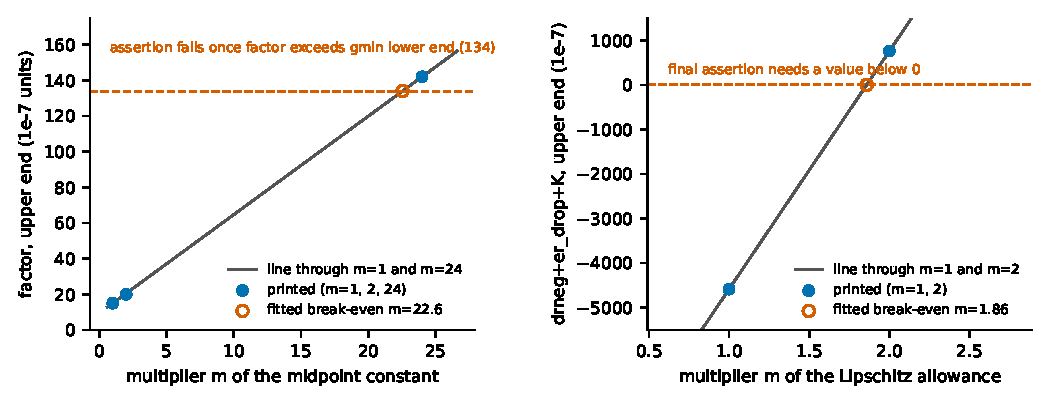
\includegraphics[width=0.96\linewidth]{gen/fig_dose.pdf}
\caption{\tier{X} Dose-response of the two thin margins. Left: upper end of \texttt{factor} against the multiplier of the midpoint constant; $m=1,2,24$ are printed values, the line passes through $m=1$ and $m=24$ (so it predicts $\SSAFactorAPred$ at $m=2$, observed $\SSAFactorAObs$) and crosses the lower end of gmin (134) at the fitted $m\approx\SSAMstar$. Right: upper end of the final left side against the multiplier of the Lipschitz allowance: $-\SSASlack$ at $m=1$, $\SSABObs$ at $m=2$ (predicted $\SSABPred$), fitted break-even $\SSAMdrop$. The break-even points are \emph{fitted} to coarsened printed pairs (the S1-neg numbers were known when the multipliers were estimated; the right panel has two points), not blind predictions.}\label{fig:dose}
\end{figure}

\emph{Margins.} Written down before A and B finished (\texttt{predictions\_AB.txt}, 20:43:39 UTC): A passes with $\texttt{factor}_{hi}\approx20$--21 (observed \SSAFactorAObs); B fails with a final left side $\approx-4585+5343=+758$ (observed \SSABObs). The midpoint constant therefore survives a loosening of about $\times\SSAMstar$ ($\texttt{er0}\approx\SSAErMid$, $\texttt{eri}\approx\SSAErInt$ in these units), whereas the Lipschitz allowance \texttt{er\_drop} (\SSAAllow{} against a slack of \SSASlack) survives only about $\times\SSAMdrop$.
The audit therefore re-derived that step (Section~\ref{sec:audit}) and found its two terms correct as stated. This is an observation about thinness, not a defect.

\subsection{Independent re-computation of the analytic constants \tier{X, SSA-X-0003, SSA-X-0004, SSA-X-0005}}
Without the C++, (a) the exact identity~(\ref{eq:cal}) can be tested: the printed $\lambda,\mu,K$ give $6K+\lambda+2\pi\mu\in[\SSACalLo,\SSACalHi]$ (exact Fractions, width \SSACalWidth), which contains $W(E_\triangle)=\SSAWtri$ computed both from the BS2018 closed form and from an Ewald sum (they differ by \SSAEwaldDiff). Positive controls: the SS-normalized Ewald values \SSASSTri{} (triangular) and \SSASSSq{} (square) match SS2012 Remark~1.5 ($\approx-0.2011$, $-0.1958$) \tier{L}, and $C$ from BS Theorem~1.5 equals $C_{\rm BHS}$ to \SSACdiff. Negative controls, all outside the interval: the square lattice (\SSANegSquare), no $2\pi$ scaling (\SSANegNoTwoPi), the $\tfrac14\log2\pi$ shift dropped (\SSANegShift). \emph{This check is blind to $\lambda$ and $\mu$:} each of the six regular sectors has area $1/6$ ($=p\,x_0$) and angle $\pi/3$ (the manuscript's Lemma K7), so the contribution of a sector is $K+\lambda/6+\mu\pi/3$, the sum over six sectors is $6K+\lambda+2\pi\mu$, and the $\lambda$ and $\mu$ terms of $K$ cancel exactly.
(b) We therefore re-implemented $f_0$, $e$, $G$, $\lambda$, $\mu$, $K$ from the TeX formulas only (mpmath, 45-digit Gauss--Legendre): $\lambda=\SSAReLam$, $\mu=\SSAReMu$, $K=\SSAReK$, each inside the certificate's printed pair, with $|G(p,x_0)|=\SSAReG$ (a positive control: $G(p,x_0)=0$ by the definition of $\mu$, so a value this small is the expected outcome) and identity residual $6K+\lambda+2\pi\mu-W(E_\triangle)=\SSAReId$. Negative controls fall outside: without the angular term $\lambda=\SSAReNoAngLam$, $K=\SSAReNoAngK$; with mode $m=1$ dropped $\lambda=\SSAReDropLam$, $K=\SSAReDropK$ (positive). Independently $B(\ell)=\SSABl$ (printed pair $(1.0464643,1.0464644)$), $|c_1|=\SSAClOne{}<1$; dropping $m=1$ gives \SSABlNegA, a wrong lattice scale \SSABlNegB. (c) Every hand constant of Section~5 passes in exact rational arithmetic (Step~8).
Two errors in \emph{our} scripts were caught and fixed: a mistyped compact form of the BS2018 closed form (corrected to the expanded form on p.~26), and a 25-digit tanh--sinh quadrature that cancelled catastrophically ($\lambda\approx5.5\cdot10^5$); the failed run still satisfied the identity to $3\cdot10^{-20}$, which is how we know check (a) cannot see $\lambda$.
\begin{figure}[t]\centering
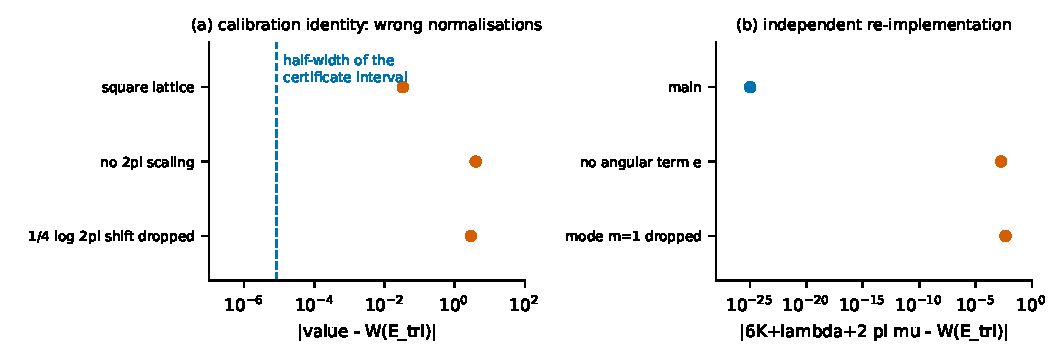
\includegraphics[width=0.96\linewidth]{gen/fig_calibration.pdf}
\caption{\tier{X} (a) Wrong normalizations of the calibration identity miss $W(E_\triangle)$ by more than three orders of magnitude more than the half-width of the certificate interval (dashed). (b) Our independent re-implementation satisfies the identity to $10^{-25}$; the two negative controls miss it by $10^{-3}$.}\label{fig:cal}
\end{figure}
This is evidence that the C++ evaluates the manuscript's formulas on $[p,R_0]$. It does not cover the spline pieces below $p$ or above $R_0$, nor the grid assertions.

\subsection{Improvement to LeanFlow: Lean data certificates, fail-closed for rendered sources \tier{A on arithmetic only; X for the tests; SSA-A-0007, SSA-X-0006, SSA-X-0007}}\label{sec:lf}
\emph{Method.} The new package \texttt{leanflow\_mcp.lean} (LeanFlow commit \hash{\SSALFCommit}, branch \texttt{\SSALFBranch}, local, not pushed; documentation \texttt{docs/LEAN\_CERTIFY.md}) turns a claim --- closed rational enclosures $x=[\mathrm{lo},\mathrm{hi}]$ and linear inequalities over their endpoints --- into one Lean theorem per assertion of the form
\lean{theorem cert\_i : (0:Int) < D $\wedge$ N * RD $\le$ RN * D := by decide}
(or \lean{norm\_num}), with all denominators cleared by Python from exact integer literals so that Lean does every multiplication and comparison. The checker compiles with a configured toolchain (timeout, optional memory cap), \emph{appends} \lean{\#print axioms cert\_i} itself, followed by a per-run random sentinel line, and requires exactly one report per theorem inside the allowlist and the sentinel exactly once after the last report; an exact \lean{Fraction} oracle is a second evaluator and any disagreement is an error.
\emph{Fail-closed behaviour.} Each of the following returns \texttt{status}$\neq$\texttt{ok}, with a test: missing toolchain, working directory or build target (including a real \lean{import} of a nonexistent module), non-zero exit, kill by signal, exit~0 with no axiom report, timeout, memory cap, \lean{sorry} warning, \lean{sorryAx} without a warning, a custom axiom, \lean{native\_decide}, a forged second axiom report, \lean{\#exit} (alone, or together with a forged report; see the audit finding below), an invalid claim (floats, injected text, $\mathrm{lo}>\mathrm{hi}$; Lean never starts), an internal exception, and Lean/oracle disagreement. False statements give \texttt{rejected} with the failing theorem names. A finding recorded in the tests: on Lean~4.34.1 \lean{native\_decide} is reported as \lean{t.\_native.native\_decide.ax\_1\_1}, not \lean{Lean.ofReduceBool}, so a classifier keyed to the old name would label it a generic custom axiom.
\emph{Results.} \texttt{pytest} gives \SSALFPassed{} passed in \SSALFPytestTime~s on the revision-stage rerun (\SSALFNotPinned{} pure-Python and core-Lean tests, including a 300-example Hypothesis property that the rendered \lean{Int} statement equals the exact \lean{Fraction} oracle, and \SSALFPinnedLog{} pinned tests on Lean~4.34.1 with Mathlib).
Applied to our runs: the \SSALFPosN{} assertions about the printed pairs of the positive run are accepted (\SSALFPosAcc{} of \SSALFPosN, axiom lists empty, \SSALFLean); for the S1-neg run \SSALFNegAcc{} of \SSALFNegN{} are accepted and \SSALFNFailed{} are rejected, exactly those containing gmin$-$factor (\SSALFFailedList).
\emph{Audit finding and fix (checker for arbitrary sources) \tier{X, SSA-X-0007}.} The independent audit (\texttt{AUDIT.md}, blocking item B2) probed the exported function \texttt{check\_lean\_source} at the pre-fix commit \hash{\SSALFOldCommit} with a source made of a custom \lean{axiom cheat : False}, a theorem \lean{(3:Int) < 2} proved from it, a forged \lean{\#eval IO.println} line imitating an axiom report, and \lean{\#exit}. \lean{\#exit} stops Lean before the appended \lean{\#print axioms}; Lean only warns ``using 'exit' to interrupt Lean'', which the checker did not reject, so the forged line was the single report and the result was \texttt{status ok, verified true} for a false statement. Controls in the same probe behaved as designed: the clean \lean{decide} proof was accepted; the cheat without \lean{\#exit} gave \texttt{custom-axiom}; the cheat with the forged line but no \lean{\#exit} gave \texttt{axiom-report-ambiguous}; the cheat with \lean{\#exit} but no forgery gave \texttt{axiom-report-missing}. The generator path \texttt{certify()} was \emph{not} affected (claim names are regex-checked, labels are single-line \texttt{--} comments; the audit's injection probe with labels \lean{/-}, \lean{-/ \#exit} and \lean{\#exit} gave \texttt{rejected}), so the 13/13 and 3/10 results above stand, and were re-run unchanged with the fixed checker (the sentinel fix is commit \hash{\SSALFFixCommit}; commit \hash{\SSALFCommit} adds only a docstring and documentation follow-up; same statuses, same accepted and rejected assertions). The fix appends a per-run random sentinel after the audit lines and requires it exactly once after the last axiom report, and also refuses the \lean{\#exit} warning (\texttt{exit-command}); there are \SSALFNNew{} new tests (two with a fake toolchain, four with real Lean), and the audit's probe now returns \texttt{error / exit-command} for the forged source with the other four controls unchanged. The earlier statement in the documentation that ``the source cannot choose what is audited'' was too strong and has been corrected. \emph{Residual scope:} Lean's \lean{\#eval} runs code, so this is a strong check but not a sandbox: a source written to defeat it could read back the temporary file and reproduce the sentinel, or redefine command syntax or elaborators (\lean{macro\_rules}, \lean{elab\_rules}) to forge the output; we therefore claim fail-closed behaviour only for sources rendered by the generator, and treat the checker as defence in depth for foreign sources.
\emph{Scope.} Tier~A covers the arithmetic on the printed outward-rounded integers, not that the C++ computed them (\tier{C, SSA-C-0005}); a failed \lean{decide} is a rejection, not a kernel-checked negation of anything about the manuscript, so it is filed at Tier~X. A toolchain that lies cannot be detected: the toolchain path is trusted configuration; real-Lean tests skip with a stated reason if the toolchain is absent; the pinned fixture needs about 78~s on a cold cache.

\section{Audit of the reduction and the certificate}\label{sec:audit}
\emph{Method and verdict \tier{C, SSA-C-0002}.} An AI agent read the manuscript sections (their sha256 values are in \texttt{REDUCTION\_AUDIT.md}), re-derived each step, classified it CONFIRMED / GAP / CANNOT\_ASSESS, and compared each certificate stage with the inequality and the constants it must certify.
\textbf{Verdict: no step of Sections 2--5 was classified as a gap.} Counts: \SSAnR{} steps for Section~2 (R1--R10), \SSAnG{} for Section~3 (G1--G7), \SSAnK{} for Section~4 (K1--K8), \SSAnT{} for Section~5 (T1--T6), and 14 certificate-stage rows, all CONFIRMED. One context citation is CONFIRMED\_WITH\_MINOR\_FIX: the manuscript's pin of Lieb--Rougerie--Yngvason ``Lemma~3 and Appendix~A'' does not match the numbering of arXiv:1701.09064v3 (the content is eq.~(3.53) and Proposition~4.2); it is context only.
Three observations that are not defects: the strip estimate is $o(t^2/\log t)$, which is exactly what makes the $n\log n$ error $o(t^2)$ (Step~3); SS2012 Lemma~4.7's proof ends with $2W$ rather than $W$ on p.~39, a factor the manuscript notes and its weakening covers; and the C++ midpoint error $H^3|A[2]|/12$ with $A[2]=Y''/2$ equals the manuscript's $(u-v)^3\sup|Y''|/24$, so there is no factor-2 discrepancy.

\emph{The thinnest point.} The negative-part assertion's Lipschitz allowance $\texttt{er\_drop}\le5343\cdot10^{-7}$ is spent against a slack of $4585\cdot10^{-7}$. The audit re-derived both terms: $\max(0,-y)$ is 1-Lipschitz and $|\partial_sG|\le L_2$, so the midpoint error per cell is $L_2h^2/4$, giving $0.65\,S_hL_2/4$; moving to the nearest $d$-node costs at most $0.65\,L_1D_h/2$. They are correct as stated, and the code matches. Our Variant~B shows the margin is real: doubling the allowance breaks the certificate.

\begin{table}[t]\centering\small
\caption{Load-bearing citations: statements read on the stated page \tier{L}; proofs are not re-checked.}\label{tab:cit}
\begin{tabular}{p{4.2cm}p{4.0cm}p{2.2cm}p{2.8cm}}\toprule used for & statement & source & read at\\\midrule
$\min_{\mathcal A_1}W$ achieved, finite; square-periodic minimizing sequence & Thm 1(3),(4) & SS2012 p.~5 & paper stage (SSA-L-0001)\\
mass displacement, one $g$ for every $\chi$ & Prop.\ 4.9 (4.12) & SS2012 p.~41 & paper stage (SSA-L-0002)\\
periodic $j$ minimized by $j_\Lambda$; scaling (1.9) & Prop.\ 3.1; Remark 7 & SS2012 pp.~26, 3 & paper stage (SSA-L-0003)\\
local $L^r$ bound & Lemma 4.7 & SS2012 pp.~38--39 & audit stage only\\
$C=\frac1\pi\min W+\frac{\log\pi}2+\log2$; value $-4.1504128$ & Thm 1.5, Thm 7.7, (2.4) & BS2018 pp.~3, 4, 26 & paper stage (SSA-L-0004)\\
$C_{\log,2}$ & Conj.\ 4 & BHS2012 p.~13 & paper stage (SSA-L-0005)\\\bottomrule\end{tabular}
\end{table}

\paragraph{Not assessable (limits of the audit) \tier{C, SSA-C-0004}.}
\begin{itemize}
\item \emph{Code $\leftrightarrow$ formula equivalence is not exhaustive.} The spline pieces on $[b,p)$ and $(R_0,l]$ (inner $S$-cutoff, $P/Q$ extension, $\tau$ blending) and the grid-stage values (gmin, drneg, the $L_1$--$L_4$ hulls, the Hessian hulls) rest on code reading; jet \texttt{pow}/\texttt{log}/\texttt{sqrt}, \texttt{cpol} and \texttt{hor} were not read line by line. No independent recomputation covers them.
\item \emph{Runtime trust} (compiler, Boost, OpenMP, hardware). Our reproduction used a different toolchain and obtained the same integers, which is not a formal guarantee.
\item \emph{Internal proofs} of SS2012 Theorem~1, Lemma~4.7, Proposition~4.9 and BS2018 Theorem~1.5 are taken as cited.
\item \emph{Negative-control coverage:} no control exercised \texttt{inside\_hess}, \texttt{calcLam} or \texttt{core\_test}; a planted Hessian-breaking edit is still owed.
\item \emph{Check blindness:} the calibration identity is blind to $\lambda$ and $\mu$; this is why check (b) of Section~\ref{sec:num} was added.
\item \emph{Uncited tool:} the strong minimum principle for $W^{2,2}_{\rm loc}$ supersolutions used in the separation lemma is standard but the manuscript gives no reference and we verified none. The independent audit located two published analogues, read on the cited pages of arXiv:1701.09064v3 (Lieb--Rougerie--Yngvason): the proof of their Proposition~4.2 (p.~21) uses the same superharmonic-minimum argument and refers to Lieb--Loss, \emph{Analysis}, Chapter~9 (which nobody here checked), and their Lemma~4.4 (p.~22, minimal distance $\ge1/\sqrt\pi$) is the closest published analogue of the separation lemma \tier{L, audit reading only; not in the ledger}. The manuscript's own pin (``Lemma~3 and Appendix~A'') could be replaced by eq.~(3.53) (p.~20), Proposition~4.2 (p.~21) and Lemma~4.4 (p.~22), as read by the auditor.
\item Section~7 (the corollary normalization) was checked at the level of the cited statements and the scaling re-derivation only.
\end{itemize}

\section{Claim ledger}\label{sec:ledger}
\texttt{ledger/build\_ledger.py} files \SSALedgerN{} claims: \SSALedgerA{} at Tier~A, \SSALedgerL{} at L, \SSALedgerC{} at C and \SSALedgerX{} at X, each with a content-addressed evidence blob in \texttt{ledger/evidence/}: verbatim axiom lines and source hashes (A), verbatim excerpts in \texttt{ledger/sources/excerpts.json} (L), the argument text and its file hash (C), result files with \texttt{claim\_licence: false} (X). Dependency edges respect the gate: A and L rows rest on nothing, the audit row (C) rests only on L rows and never on an X row, and the numerical rows rest on the scope rows.
The Elenchus gate (\texttt{tools/ledger.py ledger.json -{}-evidence-dir evidence}, output in \texttt{ledger/gate\_output.txt}) exits with code~\SSAGateExit. It reports \textbf{\SSAGateBlock{} blocking findings} and \textbf{\SSAGateFlag{} flags}, all \texttt{LEDGER\_UNAUDITED\_TIER\_A}: no person has certified that the Tier~A statements mean what their glosses say. The flags remain open. \texttt{elenchus\_check.py} works on Lean files only and was not applicable; \texttt{citation\_check.py} was run at the revision stage, on \texttt{pdftotext} output of the arXiv PDFs of SS2012 (v2) and BS2018 (v5) (\texttt{data/citation\_check/}), for five theorem-type rows (SS Theorem~1 items 3--4, Theorem~2, Proposition~3.1, Proposition~4.9; BS Theorem~1.5): the verbatim passages are \texttt{ACCEPTED} (the quote is present in the primary text, statement and hypotheses listed; \texttt{statement\_match} is our judgment), while the ledger's own excerpts are \texttt{REFUSED} because they are rejoined ASCII transcriptions of the alphaXiv extraction, not verbatim primary text, and two one-word tampers of real quotes are \texttt{REFUSED}. So the ledger's L rows are faithful transcriptions in content, not verbatim quotations; the tool does not check that a statement means what we say, and the conjectures (SS Conjecture~1, BHS Conjecture~4) and the BS value formula are outside its scope (they remain read-on-the-page claims by the auditor and the paper-stage agent).

\section{Limitations}\label{sec:lim}
\begin{itemize}
\item \textbf{Conditionality.} Every statement about the truth of the conjecture rests on the openai/math manuscript (AI-generated, not peer reviewed), on cited literature whose proofs we did not re-check, and on a computer run whose runtime is trusted.
\item \textbf{Same-pipeline verification.} Producer, auditor, Lean author and paper-stage agent are AI instances of the same pipeline; re-compilations are not producer$\neq$verifier. No human has audited the Lean statements, the audit, or this paper.
\item \textbf{The Lean statements are not proofs.} The ten lemmas only show that the definitions are not degenerate. The competitor class, the existence of the puncture limit and the triangular side's inhabitation are open points (Section~\ref{sec:lean}); a subtle misstatement would not be caught by any Lean check.
\item \textbf{Reproduction scope.} One run each, on cores 0--3 or 4--7 of one host; the wrapper's 32-thread setting oversubscribed four cores; no test of the analytic bounds the certificate depends on.
\item \textbf{Control coverage and fitted margins.} The loosened copies change one constant each; the break-even multipliers are fitted to coarsened pairs and not blind; no control reaches \texttt{inside\_hess}.
\item \textbf{Independent audit and revision.} A second agent instance of the same pipeline audited this preprint before publication (verdict: accept with corrections; \texttt{AUDIT.md}); the corrections are listed in \texttt{REVISION.md}. Its open items remain open: no planted Hessian-breaking control, and no independent check of the spline pieces outside $[p,R_0]$ or of the grid-stage values.
\item \textbf{LeanFlow checker scope.} Fail-closed behaviour is claimed only for sources rendered by the generator; the checker for arbitrary Lean sources is not a sandbox (Section~\ref{sec:lf}).
\item \textbf{Audit depth.} Section~\ref{sec:audit}. In particular, \texttt{CONFIRMED} means the audit agent found no error, not that none exists.
\item \textbf{Literature.} We did not search for work on the conjecture after the cited papers; claims about its status are the cited sources' own.
\end{itemize}

\section{Reproducibility}\label{sec:repro}
AutoevolveAI files are uncommitted on top of \texttt{9d245742c1655852103abb28f585e21af54851e6} (branch \texttt{worktree-openai-math-discovery}). The openai/math checkout used for the corpus has HEAD \texttt{adc7f1241b42e322a6451854ab7e4b4c146bf78a}; the preprint is the folder \texttt{Triangular-minimality-for-planar-Coulomb-renormalized-energy-September-23-2026} (the four verification sources are identified by the sha256 values in Section~\ref{sec:num}). Lean sha256: statement \hash{\SSAShaMain}; controls \hash{\SSAShaCtl}. LeanFlow: commit \hash{\SSALFCommit}.
\begin{lstlisting}[basicstyle=\ttfamily\tiny]
taskset -c 4-7 python3 scripts/certified_numerics/lean_pinned.py compile formal_cert/Programmes/SandierSerfatyStatement.lean --olean Programmes.SandierSerfatyStatement --json-out papers/prog_sandier_serfaty_audit/rerun/compile_statement.json
taskset -c 4-7 python3 scripts/certified_numerics/lean_pinned.py compile formal_cert/Programmes/SandierSerfatyStatementControls.lean --json-out papers/prog_sandier_serfaty_audit/rerun/compile_controls.json
.venv/bin/python -I results/programmes/2026-10-25/P1/s3/statement_lock.py check
python3 -I -B run-certificate.py --output-dir <fresh dir>          # in the corpus verification/ folder, on a fresh directory; wrapper hard-codes OMP_NUM_THREADS=32
cd <LeanFlow worktree>; AutoevolveAI/.venv/bin/python -I -m pytest -c pyproject.toml tests -q -p no:cacheprovider
.venv/bin/python -I papers/prog_sandier_serfaty_audit/ledger/build_ledger.py; .venv/bin/python -I papers/prog_sandier_serfaty_audit/ledger/run_gate.py
.venv/bin/python -I papers/prog_sandier_serfaty_audit/gen_inputs.py; pdflatex main.tex (twice)
\end{lstlisting}
All data used by the paper (receipts, logs, patches, predictions, audit scripts and outputs, Lean transcripts) are copied into \texttt{papers/prog\_sandier\_serfaty\_audit/data/}; the ledger evidence blobs hash them. \emph{Paper-stage reruns} (same AI pipeline, not an independent verifier \tier{X, SSA-X-0008}): Lean recompile of the statement (\SSACompileMain) and controls (\SSACompileCtl), lock check \texttt{\SSALockCheck}, LeanFlow \SSALFPassed{} tests passed (after the checker fix; the pre-fix run, 82 tests at commit \hash{\SSALFOldCommit}, is kept as \texttt{rerun/leanflow\_pytest\_before\_fix\_commit542cea9.txt}). The revision changed the docstring of the Lean file (hash before: \hash{\SSAShaMainOld}; the locked statement-region hash is unchanged) and the pre-revision files are kept in \texttt{data/before\_revision/}.

\begin{thebibliography}{99}\small
\bibitem{ss} E.~Sandier, S.~Serfaty, \emph{From the Ginzburg--Landau model to vortex lattice problems}, Comm.\ Math.\ Phys.\ \textbf{313} (2012) 635--743; arXiv:1011.4617v2.
\bibitem{bs} L.~B\'etermin, E.~Sandier, \emph{Renormalized energy and asymptotic expansion of optimal logarithmic energy on the sphere}, arXiv:1404.4485v5 (2018).
\bibitem{bhs} J.~S. Brauchart, D.~P. Hardin, E.~B. Saff, \emph{The next-order term for optimal Riesz and logarithmic energy asymptotics on the sphere}, Contemp.\ Math.\ \textbf{578} (2012) 31--61; arXiv:1202.4037v1 (the page numbers cited are those of the arXiv version).
\bibitem{oai} OpenAI, \emph{Triangular minimality for planar Coulomb renormalized energy} (preprint dated 2026-09-23), in the OpenAI Math release, github.com/openai/math (checkout HEAD \texttt{adc7f124\ldots}), folder \texttt{preprints/Triangular-minimality-for-planar-Coulomb-renormalized-energy-September-23-2026}. AI-generated; not peer reviewed.
\bibitem{txt} X.~Callens, \emph{The Triangular Lattice and Universal Optimality} (textbook), doi:10.5281/zenodo.23295142 (2026).
\bibitem{ar} X.~Callens, five sibling preprints applying the same approach (kernel-checked consequences of the same openai/math release for explicit interactions, with Elenchus-tiered claims): bilayer dipolar excitons doi:10.5281/zenodo.23646103, Yukawa crystals doi:10.5281/zenodo.23646105, Rytova--Keldysh doi:10.5281/zenodo.23646107, $\sigma=3$ dyadic enstrophy doi:10.5281/zenodo.23646111, Bogoliubov structure factor doi:10.5281/zenodo.23646117 (DOIs reserved on the title pages at the time of writing).
\end{thebibliography}
\noindent This preprint applies the tiered approach of~\cite{txt,ar} to a claim about a different problem: here the openai/math result is the object of audit rather than an input.
\end{document}
